\section{图的覆叠空间}
\label{ch14-sec83}

我们现在来定义线性图 (有限情形前面已介绍过), 并且证明下面的基本定理: 线性图的覆叠空间也是线性图.

让我们来回顾一下: 弧 $A$ 是同胚于单位区间 $[0,\ 1]$ 的空间, 弧 $A$ 的\textbf{端点} $p$ 和 $q$ 是在同胚下对应着 $0$ 和 $1$ 的那两个点, 只有这两个点能使 $A-p$ 和 $A-q$ 是连通的. 弧 $A$ 的\textbf{内部}是从 $A$ 中除掉了端点后的剩余部分.

\begin{definition}[线性图]
\label{definition:ch14-linear-graph}
一个\textbf{线性图}(linear graph) $X$ 是由一些弧 $A_{\alpha}$ 构成的一个族的并, 要求满足条件:
\begin{enumerate}[(1)]
\item 两条弧的交 $A_{\alpha}\cap A_{\beta}$ 或者是空的, 或者是这两条弧的一个公共端点.
\item $X$ 的拓扑与这些子空间 $A_{\alpha}$ 相通.
\end{enumerate}
这些弧 $A_{\alpha}$ 叫做 $X$ 的\textbf{边}(edge), 这些弧的内部则叫做 $X$ 的\textbf{开边}(open edge). 这些弧的端点叫做 $X$ 的\textbf{顶点}(vertex). 由 $X$ 的顶点构成的集合记作 $X^{0}$.
\end{definition}

设 $X$ 是一个线性图. 如果子集 $C$ 是 $X$ 的某些边和某些顶点的并, 则它是 $X$ 的一个闭子集. 这是因为 $C$ 与 $A_{\alpha}$ 的交要么是空集, 要么等于 $A_{\alpha}$, 要么等于 $A_{\alpha}$ 的一个或两个顶点, 无论何种情形 $C\cap A_{\alpha}$ 在 $A_{\alpha}$ 中都是闭的. 由此可见 $X$ 的每一条边都是闭集, 也可见 $X^{0}$ 是 $X$ 的一个闭的离散子空间, 因为 $X^{0}$ 的任何子集在 $X$ 中都是闭的.

对于前面对论的有限线性图的情形, 我们当时在定义中用了一个 Hausdorff 条件替代条件 (2). 那时, 这个 Hausdorff 条件可以保证 $X$ 的拓扑与诸子空间是相通的. 但对于无限图的情形不再成立, 所以我们要把相通条件作为定义的一部分. 当然可以还加上 Hausdorff 条件, 但是已经没有必要了, 因为它被相通条件所蕴涵.

\begin{lemma}[线性图是正则空间]
\label{lemma:ch14-graph-regular}
每一个线性图都是正则空间, 因此当然也是一个 Hausdorff 空间.
\end{lemma}

\begin{proof}
设 $B$ 和 $C$ 是 $X$ 的两个无交闭子集. 不失一般性, 假定 $X$ 的每一个顶点要么属于 $B$, 要么属于 $C$. 对于每一个 $\alpha$, 选取 $A_{\alpha}$ 的两个无交子集 $U_{\alpha}$ 和 $V_{\alpha}$ 分别包含着 $B\cap A_{\alpha}$ 和 $C\cap A_{\alpha}$, 并且要求 $U_{\alpha}$ 和 $V_{\alpha}$ 在 $A_{\alpha}$ 中都是开的. 令 $U=\bigcup U_{\alpha}$ 和 $V=\bigcup V_{\alpha}$, 此时 $U$ 和 $V$ 分别包含 $B$ 和 $C$.

我们来证明 $U$ 和 $V$ 是无交的. 如果 $x\in U\cap V$, 则 $x\in U_{\alpha}\cap V_{\beta}$ 对于 $\alpha\neq\beta$ 成立. 这表明 $A_{\alpha}$ 和 $A_{\beta}$ 都要包含点 $x$, 从而 $x$ 是 $X$ 的一个顶点. 但这是不可能的, 因为如果 $x\in B$, 则 $x$ 便不会在任何一个集合 $V_{\beta}$ 中. 如果 $x\in C$, 那么 $x$ 便不会在任何一个集合 $U_{\alpha}$ 中.

最后证明 $U$ 和 $V$ 都是 $X$ 中的开集. 为了证明 $U$ 是开的, 只需证明对于每一个 $\alpha$, $U\cap A_{\alpha}=U_{\alpha}$. 根据定义, $U\cap A_{\alpha}$ 包含着 $U_{\alpha}$. 如果 $x$ 是 $U\cap A_{\alpha}$ 中的一个不在 $U_{\alpha}$ 中的点, 则对于某一个 $\beta\neq\alpha$, $x$ 属于 $U_{\beta}$. 于是 $A_{\beta}$ 和 $A_{\alpha}$ 都包含 $x$, 从而 $x$ 是 $X$ 的一个顶点. 然而这是不可能的, 因为如果 $x\in B$, 则根据 $U_{\alpha}$ 的定义, $x\in U_{\alpha}$. 如果 $x\in C$, 则 $x$ 不能属于 $U$.
\end{proof}

\par
\begin{figure}[htbp]
\centering
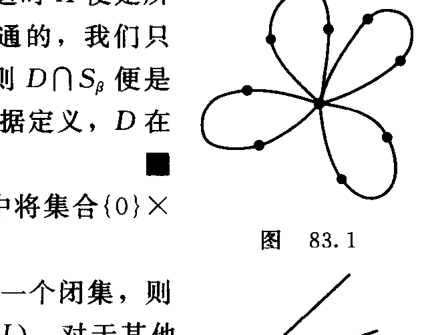
\includegraphics[width=0.4\textwidth]{image/fig-83-1.png}
\caption{圆周束作为线性图.}
\label{ch14-fig-83-1}
\end{figure}

\begin{example}[圆周束是线性图]
\label{example:ch14-wedge-linear}
如果 $X$ 是某些圆周 $S_{\alpha}$ 的束, 其公共点为 $p$, 则 $X$ 可以表示为线性图. 我们只要把每一个 $S_{\alpha}$ 表示成以 $p$ 为一个顶点的具有三条边的一个图, 这时 $X$ 便是所有弧的并了. 为了证明束 $X$ 的拓扑与这些弧的一个族是相通的, 我们只要注意: 如果对于每一段弧 $A_{\alpha}$, $D\cap A_{\alpha}$ 是 $A_{\alpha}$ 中的闭集, 则 $D\cap S_{\beta}$ 便是形如 $D\cap A_{\alpha}$ 的三个闭集之并, 从而在 $S_{\beta}$ 中是闭的. 因此根据定义, $D$ 在 $X$ 中是闭的. 参见\cref{ch14-fig-83-1}.

\end{example}

\par
\begin{figure}[htbp]
\centering
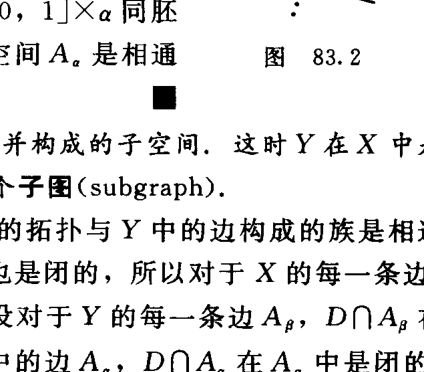
\includegraphics[width=0.4\textwidth]{image/fig-83-2.png}
\caption{无限星形线性图.}
\label{ch14-fig-83-2}
\end{figure}

\begin{example}[无限星是线性图]
\label{example:ch14-infinite-star}
设 $J$ 是一个离散空间, $E=[0,\ 1]\times J$, 则在 $E$ 中将集合 $\{0\}\times J$ 缩成一点 $p$ 所得到的商空间是一个线性图.

商映射 $\pi\colon E\to X$ 是一个闭映射. 因为如果 $C$ 是 $E$ 中的一个闭集, 则当 $C$ 包含着 $\{0\}\times J$ 的一个点时, $\pi^{-1}\pi(C)$ 等于 $C\cup(\{0\}\times J)$. 对于其他情形, $\pi^{-1}\pi(C)$ 等于 $C$. 在任何一种情形下, $\pi^{-1}\pi(C)$ 在 $E$ 中都是闭的, 因此 $\pi(C)$ 是 $X$ 中的一个闭集. 这蕴涵着 $\pi$ 将每一个空间 $[0,\ 1]\times\alpha$ 同胚地映为它的像 $A_{\alpha}$, 所以 $A_{\alpha}$ 是一段弧. $X$ 的拓扑与这些子空间 $A_{\alpha}$ 是相通的, 因为 $\pi$ 是一个商映射. 参见\cref{ch14-fig-83-2}.

\end{example}

\begin{definition}[子图]
\label{definition:ch14-subgraph}
设 $X$ 是一个线性图, $Y$ 为 $X$ 中由 $X$ 的一些边的并构成的子空间. 这时 $Y$ 在 $X$ 中是闭的, 并且它自己也是一个线性图, 我们将它称为 $X$ 的一个\textbf{子图}(subgraph).
\end{definition}

为了证明 $Y$ 是一个线性图, 我们要指出 $Y$ 作为子空间的拓扑与 $Y$ 中边构成的族是相通的. 如果 $Y$ 的子集 $D$ 在子空间 $Y$ 中是闭的, 则 $D$ 在 $X$ 中也是闭的, 所以对于 $X$ 的每一条边, 特别对于 $Y$ 的每一条边, $D\cap A_{\alpha}$ 在 $A_{\alpha}$ 中是闭的. 反之, 设对于 $Y$ 的每一条边 $A_{\beta}$, $D\cap A_{\beta}$ 在 $A_{\beta}$ 中是闭的. 我们还要指出的是对于 $X$ 的每一条不在 $Y$ 中的边 $A_{\alpha}$, $D\cap A_{\alpha}$ 在 $A_{\alpha}$ 中是闭的. 然而此时, $D\cap A_{\alpha}$ 或者是空的, 或者是一个单点集! 这便证明了 $Y$ 的拓扑与它的所有边相通.

\begin{lemma}[紧致子集含于有限子图]
\label{lemma:ch14-compact-finite-subgraph}
设 $X$ 是一个线性图. 如果 $C$ 是 $X$ 的一个紧致子空间, 则 $X$ 中存在着一个有限子图 $Y$ 包含着 $C$. 如果 $C$ 是连通的, 则 $Y$ 也可以选成连通的.
\end{lemma}

\begin{proof}
首先, 我们注意 $C$ 仅包含着 $X$ 中的有限个顶点. 因为 $C\cap X^{0}$ 是一个紧致空间 $C$ 的闭离散子空间, 且由于它没有极限点, 所以这个子空间必是有限的. 类似地, 只有有限多个 $\alpha$ 使得 $C$ 包含边 $A_{\alpha}$ 的一个内点. 因为如果对于每一个 $\alpha$, 只要可能, 选取 $C$ 中的一个 $A_{\alpha}$ 的内点 $x_{\alpha}$, 那么我们便得到了一个集合 $B=\{x_{\alpha}\}$, 它与每一条边 $A_{\beta}$ 之交是单点集或空集. 由此可见, $B$ 的每一个子集在 $X$ 中都是闭的, 所以 $B$ 是 $C$ 中的闭离散子空间, 因此是有限的.

对于 $X$ 中每一个属于 $C$ 的顶点 $x$, 选取以 $x$ 为顶点的一条边, 再选取那些内部包含着 $C$ 中的点的边 $A_{\alpha}$. 令 $Y$ 为所有这些边的并, 它便是包含着 $C$ 的一个有限子图. 注意如果 $C$ 是连通的, 则 $Y$ 便是与 $C$ 有交的弧的一个族的并, 因此 $Y$ 是连通的.
\end{proof}

\begin{lemma}[线性图局部道路连通且半局部单连通]
\label{lemma:ch14-graph-locally}
如果 $X$ 是一个线性图, 则 $X$ 是局部道路连通的和半局部单连通的.
\end{lemma}

\begin{proof}
\textbf{第一步.} 我们证明 $X$ 是局部道路连通的. 如果 $x\in X$ 并且 $x$ 在 $X$ 的某一条边的内部, 则 $x$ 的每一个邻域中包含着 $x$ 的一个邻域同胚于 $\mathbb{R}$ 中的一个开区间, 而开区间是道路连通的. 另一方面, 如果 $x$ 是 $X$ 的一个顶点, 而 $U$ 是 $x$ 的一个邻域, 则对于以 $x$ 为端点的每一条边 $A_{\alpha}$, 我们可以选取 $x$ 在 $A_{\alpha}$ 中的一个邻域 $V_{\alpha}$ 包含在 $U$ 中, 并且要求这个邻域同胚于半开区间 $[0,\ 1)$. 于是 $\bigcup V_{\alpha}$ 是 $x$ 在 $X$ 中的一个包含于 $U$ 中的邻域, $x$ 的这个邻域是一些道路连通空间之并, 这些道路连通空间有一个公共点 $x$.

\textbf{第二步.} 我们来证明 $X$ 是半局部单连通的. 事实上, 要证明的是如果 $x\in X$, 则 $x$ 有一个邻域 $U$ 使得 $\pi_{1}(U,\ x)$ 是平凡的.

如果 $x$ 在 $X$ 的某一条边的内部, 那么这个内部便是这样一个邻域. 现在假设 $x$ 是 $X$ 的一个顶点. 用 $\overline{\mathrm{St}}\,x$ 表示 $X$ 中那些以 $x$ 为端点的边的并, 用 $\mathrm{St}\,x$ 表示从 $\overline{\mathrm{St}}\,x$ 中除掉所有异于 $x$ 的那些顶点剩下的部分. ($\mathrm{St}\,x$ 叫做 $x$ 的\textbf{星}.) 集合 $\mathrm{St}\,x$ 是 $X$ 中的开集, 因为它是一些弧和一些顶点的并的补. 我们来证明 $\pi_{1}(\mathrm{St}\,x,\ x)$ 是平凡的.

设 $f$ 是 $\mathrm{St}\,x$ 中以 $x$ 为基点的一条回路, 则像集 $f(I)$ 是紧致的, 所以它在 $\overline{\mathrm{St}}\,x$ 的有限条弧的并中. 任何一个这样的并都同胚于平面上有限条具有一个公共端点的线段之并. 在这种空间中的任何一条回路都可经由直线同伦收缩到 $x$ 处的常值回路.

如果 $x$ 是 $X$ 的一个顶点, 这时单点空间 $\{x\}$ 是 $\overline{\mathrm{St}}\,x$ 的一个形变收缩核. 然而, 尽管所需要的形变收缩容易想得到, 但证明这个映射的连续性却并不容易. 我们需要以下事实: 如果将映射
\[
F\colon(\overline{\mathrm{St}}\,x)\times I\longrightarrow\overline{\mathrm{St}}\,x
\]
限制在每一个子空间 $A_{\alpha}\times I$ 上是连续的, 那么这个映射本身便是连续的. 当 $\overline{\mathrm{St}}\,x$ 是有限多条弧的并时, 这个结论立刻便能从黏结引理推出, 而一般性的结论要求我们证明 $(\overline{\mathrm{St}}\,x)\times I$ 的拓扑与子空间 $A_{\alpha}\times I$ 是相通的. 这可从关于商映射乘积的一个基本定理得到. (参见第 29 节中的习题 11.) 如果我们只想将一条回路 (而不是将整个空间 $\overline{\mathrm{St}}\,x$) 收缩为一点, 则无需这些考虑, 因为任何一条回路都包含在有限条边的并中, 收缩成一点是不成问题的.
\end{proof}

现在来考虑线性图的覆叠空间. 在上一章中我们约定每一个覆叠空间都是道路连通和局部道路连通的, 现在解除这个约定.

\begin{theorem}[线性图的覆叠空间仍是线性图]
\label{theorem:ch14-covering-of-graph}
设 $p\colon E\to X$ 是一个覆叠映射, 其中 $X$ 是一个线性图. 如果 $A_{\alpha}$ 是 $X$ 的一条边, 而 $B$ 是 $p^{-1}(A_{\alpha})$ 的一个道路分支, 则 $p$ 是从 $B$ 到 $A_{\alpha}$ 上的一个同胚. 从而空间 $E$ 也是一个线性图, 以所有空间 $p^{-1}(A_{\alpha})$ 的所有道路分支为它的边.
\end{theorem}

\begin{proof}
\textbf{第一步.} 我们来证明 $p$ 是从 $B$ 到 $A_{\alpha}$ 上的一个同胚. 由于弧 $A_{\alpha}$ 是道路连通和局部道路连通的, 定理 53.2 和 \cref{lemma:ch13-path-component-covering} 告诉我们 $p$ 的限制映射 $p_{0}\colon B\to A_{\alpha}$ 是一个覆叠映射. 由于 $B$ 是道路连通的, 所以提升对应 $\phi\colon\pi_{1}(A_{\alpha},\ a)\to p_{0}^{-1}(a)$ 是满的. 由于 $A_{\alpha}$ 是单连通的, 所以 $p_{0}^{-1}(a)$ 由一个点构成. (参见定理 54.4.) 因此 $p_{0}$ 是一个同胚.

\textbf{第二步.} 由于 $X$ 是一些弧 $A_{\alpha}$ 的并, 空间 $E$ 便是作为空间 $p^{-1}(A_{\alpha})$ 的道路分支的那些弧 $B$ 的并. 设 $B$ 和 $B'$ 分别是 $p^{-1}(A_{\alpha})$ 和 $p^{-1}(A_{\beta})$ 的道路分支, $B\neq B'$. 我们来证明 $B$ 和 $B'$ 最多相交于一个公共端点. 如果 $A_{\alpha}$ 和 $A_{\beta}$ 是相等的, 则 $B$ 和 $B'$ 是无交的. 如果 $A_{\alpha}$ 和 $A_{\beta}$ 是无交的, 则 $B$ 和 $B'$ 也是无交的. 从而, 如果 $B$ 和 $B'$ 相交, $A_{\alpha}$ 和 $A_{\beta}$ 应当相交于二者的一个公共端点, 因此 $B\cap B'$ 中只有一个点, 它应当既是 $B$ 的端点也是 $B'$ 的端点.

\textbf{第三步.} 我们证明 $E$ 的拓扑与它的那些弧 $B$ 相通. 这是这个定理证明中最难的部分. 设 $W$ 是 $E$ 的一个子集, 使得对于 $E$ 中的每一条弧 $B$, $W\cap B$ 在 $B$ 中是开的. 我们来证明 $W$ 是 $E$ 中的一个开集.

首先, 证明 $p(W)$ 在 $X$ 中是开的. 如果 $A_{\alpha}$ 是 $X$ 的一条边, 则 $p(W)\cap A_{\alpha}$ 便是集合 $p(W\cap B)$ 的并, 其中 $B$ 取遍 $p^{-1}(A_{\alpha})$ 的所有道路分支. 这些集合 $p(W\cap B)$ 中的每一个在 $A_{\alpha}$ 中是开的, 这是因为 $p$ 将 $B$ 同胚地映射到 $A_{\alpha}$ 上. 因此这些集合的并 $p(W)\cap A_{\alpha}$ 也是 $A_{\alpha}$ 中的开集. 由于 $X$ 的拓扑与子空间 $A_{\alpha}$ 相通, 所以集合 $p(W)$ 是 $X$ 中的开集.

其次, 取一个特殊情形来证明我们的结论. 这个特殊情形是: $X$ 中有一个被 $p$ 均衡地覆盖着的开集 $U$, 使得 $W$ 包含在 $p^{-1}(U)$ 的某一片 $V$ 中. 这时, 根据刚才证明的结论可见, 集合 $p(W)$ 在 $X$ 中是开的. 这蕴涵着 $p(W)$ 是 $U$ 中的开集. 由于 $p$ 的限制映射是从 $V$ 到 $U$ 上的同胚, 所以 $W$ 也是 $V$ 中的开集, 因此它在 $E$ 中也是开的.

最后, 我们证明一般结论. 选取 $X$ 的一个覆盖 $\mathcal{A}$, 它由被 $p$ 均衡地覆盖着的开集 $U$ 组成. 这时, 取遍所有 $U\in\mathcal{A}$, 集合 $p^{-1}(U)$ 中的所有片 $V$ 覆盖着 $E$. 对于每一个这样的片 $V$, 令 $W_{V}=W\cap V$. 集合 $W_{V}=W\cap V$ 满足条件: 对于 $E$ 中的每一条弧 $B$, 集合 $W_{V}\cap B$ 在 $B$ 中是开的, 这是因为 $W_{V}\cap B=(W\cap B)\cap(V\cap B)$, 而两个集合 $W\cap B$ 和 $V\cap B$ 在 $B$ 中都是开的. 前一段中的结论蕴涵着 $W_{V}$ 在 $E$ 中是开的. 由于 $W$ 是集合 $W_{V}$ 的并, 所以它在 $E$ 中也是开的.
\end{proof}

\begin{exercise}
\label{exercise:ch14-sec83-01}
在证明线性图 $X$ 的正则性的过程中, 为什么要假设 $X$ 的每一个顶点属于 $B$ 和 $C$ 之一?
\end{exercise}

\begin{exercise}
\label{exercise:ch14-sec83-02}
有限线性图 $X$ 的\textbf{Euler 数}等于 $X$ 的顶点的个数减去边的个数. 我们将看到, 它是一个拓扑不变量. 计算一段弧的 Euler 数、一个圆周的 Euler 数、$n$ 个圆周束的 Euler 数以及 $n$ 个顶点的完全图的 Euler 数. 如果 $E$ 是 $X$ 的一个 $n$-重覆叠空间, $E$ 的 Euler 数和 $X$ 的 Euler 数之间有什么关系?
\end{exercise}
